% Load the kaohandt class (with the default options)
\documentclass[
	%fontsize=10pt, % Base font size
	%twoside=false, % If true, use different layouts for even and odd pages (in particular, if twoside=true, the margin column will be always on the outside)
	%secnumdepth=2, % How deep to number headings. Defaults to 2 (subsections)
	%abstract=true, % Uncomment to print the title of the abstract
]{kaohandt}

% Choose the language
\usepackage[english]{babel} % Load characters and hyphenation
\usepackage[english=british]{csquotes}	% English quotes
\usepackage{kotex}

% Load packages for testing
\usepackage{blindtext}
\usepackage{qcircuit}
%\usepackage{showframe} % Uncomment to show boxes around the text area, margin, header and footer
%\usepackage{showlabels} % Uncomment to output the content of \label commands to the document where they are used

\graphicspath{{images/}{./}} % Paths where images are looked for

% Load mathematical packages for theorems and related environments.
\usepackage{kaotheorems}

% Load the bibliography package
\usepackage{kaobiblio}
\addbibresource{report-template.bib} % Bibliography file

% Load the package for hyperreferences
\usepackage{kaorefs}
\usepackage{braket}

%----------------------------------------------------------------------------------------

\begin{document}

%----------------------------------------------------------------------------------------
%	REPORT INFORMATION
%----------------------------------------------------------------------------------------

\title[Term paper]{Term Paper (EE547) \\ \large Review of "Purification of Noisy Entanglement and Faithful Teleportation via Noisy Channels"}
\author[SV]{20244275, Vaughn Sohn}
\date{\today}

%----------------------------------------------------------------------------------------
%	TITLE AND ABSTRACT
%----------------------------------------------------------------------------------------

\maketitle

\margintoc

\begin{abstract}
\noindent
본 논문은 Alice와 Bob이라는 두 명의 분리된 관찰자가 자신의 system에 local operation을 가하는 것만으로 적은 개수의 \textbf{high purity} entangled pair를 만들 수 있음을 보인다.
\end{abstract}

% {\noindent\textbf{Keywords:} \LaTeX, Kao, handout, article, report}

\medskip

%----------------------------------------------------------------------------------------
%	MAIN BODY
%----------------------------------------------------------------------------------------

\section{Review the article}
\begin{kaobox}
    \textit{Review the article in detail. You're encouraged to reproduce the calculations.}
\end{kaobox}
\subsection{Introduction and background}

Quantum information theory에서 주로 다루는 주제인 teleportation, compression은 주어진 quantum information을 저장하거나 전송하기 위해서 얼마나 많은 자원(i.e., number of qubits)을 요구하는지를 분석한다. 
Quantum compression은 Shannon의 classical compression의 아이디어와 유사하게 von Neumman entropy를 이용하여 신뢰할 수 있는 압축을 위해 필요한 qubit의 개수를 계산할 수 있다. 
\sidenote[][*-2]{Shannon entropy:\\ \begin{equation*}
    H(P) = -\sum_i p_i \log_2 p_i
\end{equation*}}
\begin{equation}
    S(\rho)=-\operatorname{Tr} \rho \log _2 \rho, \quad \text { where } \rho=\sum_i p_i\left|\psi_i\right\rangle\left\langle\psi_i\right| .
\end{equation}

Quantum teleportation은 maximally entangled qubit을 송신자와 수신자가 공유한 뒤, local operation과 2-bit classical communication만으로도 arbitrary quantum state를 전송할 수 있는 프로토콜이다.
그러나 이러한 논의는 모두 \textbf{noiseless quantum channel}을 필요로한다. 예를 들어, quantum teleportation이 성립하기 위해서는 pure maximally entangled state를 공유할 수 있어야하지만 noise quantum channel을 이용하여 전송하면 impure한 state; \textit{mixed state}가 된다.

따라서 이를 해결하기 위해서 기존의 quantum state를 더 큰 차원의 Hilbert space로 표현하는 quantum error correction code(QEC)가 연구되고 있다. 

본 연구에서는 QEC가 아닌 다른 관점을 사용하여 2명의 서로 분리된 관찰자(Alice와 Bob이라고 하자)가 local unitary operation과 measurement, classical communication을 사용하여 더 높은 purity를 가지는 entangled pair를 얻을 수 있음을 보이고자한다. 
제안한 방법을 이용하면 거의 perfectly pure한 상태로 purification 할 수 있기 때문에 perfectly entangled pair로서 quantum teleportation에 이용될 수 있다.

\subsection{Methodology}
$M$이 two spin-$\frac{1}{2}$ 입자의 general mixed state이고, 이 state로부터 pure entanglement state $\ket{\Psi^-}$를 distillation 하려고 한다.

주어진 state에 대한 purity는 perfect singlet과의 \textbf{fidelity}를 이용하여 정의될 수 있다. 
\sidenote[][*-2]{$F$는 nonlocally 정의되었지만, two spin을 locally 측정했을 때 same random axis를 얻을 확률 $P_{\|}$을 이용하여 계산할 수 있다. \begin{equation*}
    F = 1- \frac{3 P_{\|}}{2}
\end{equation*}}
\begin{equation}
    F = \braket{\Psi^- | M | \Psi^-}
\end{equation}

Purification procedure를 이해하는 가장 쉬운 방법은 $M$이 이미 pure state인 특수한 상황을 가정하는 것이다. ($M = \ket{\Gamma} \bra{\Gamma}$)
Pure state의 entanglement는 reduced density matrix의 von Neumman entropy로 정의될 수 있다. \sidenote[][*-2]{\begin{equation*}
    E(\Gamma) = S(\rho_A) = S(\rho_B)
\end{equation*}}따라서, $n$개의 $\ket{\Gamma} \bra{\Gamma}$는 $m = n \cdot E(\Gamma)$개의 maximally entangled state; $\ket{\Psi^-}\bra{\Psi^-}$으로 표현될 수 있다. 

이제 다시 원래 문제인 \textit{mixed state}로부터 pure singlet을 얻어내는 것에 집중하자. 첫 번쨰 아이디어는 바로 Alice와 Bob이 공유하고 있는 state에 \textit{random bilateral rotation} gate를 적용하는 것이다.\sidenote[][*-2]{$SU(2)$로부터 랜덤한 local rotation gate를 선택하여 각 pair를 이루는 qubit에 동일한 gate를 적용}
이 과정을 수행하면, initial general mixed state $M$을 다음과 같은 \textit{Werner state}로 전환할 수 있다.
\sidenote[][]{Bell state: \begin{equation*}
    \ket{\Phi^{\pm}} = \frac{\ket{00} \pm \ket{11}}{\sqrt 2};\quad \ket{\Psi^{\pm}} = \frac{\ket{01} \pm \ket{10}}{\sqrt 2}
\end{equation*}}
\begin{equation}
    \begin{aligned}
        W_F & =F \left|\Psi^{-}\right\rangle\left\langle\Psi^{-}\right|+\frac{1-F}{3}\left|\Psi^{+}\right\rangle\left\langle\Psi^{+}\right| \\
        & +\frac{1-F}{3}\left|\Phi^{+}\right\rangle\left\langle\Phi^{+}\right|+\frac{1-F}{3}\left|\Phi^{-}\right\rangle\left\langle\Phi^{-}\right|
    \end{aligned}
    \label{eq:WF}
\end{equation}

Werner state는 동일한 amplitude를 갖는 3개의 triplet state, 그리고 amplitude가 $F$인 singlet state의 mixture state이다. 이는 singlet state가 \textit{bilateral rotation}에 invariance하기 때문에 만들어진다.
이렇게 얻은 $W_F$는 $\ket{\Phi^-}$와는 $F$만큼 overlap되기 때문에 여전히 fidelity $F$를 가진다. 

앞으로 본 논문에서 사용할 몇가지 local operations에 대해서 설명하고자한다. 
\begin{itemize}
    \item Unilateral Pauli rotations: entangled pair에서 하나의 입자에 대해 $\pi$ rad만큼 회전한다. (x,y, or z axis)\sidenote[][]{각 Bell state에 대해 1-to-1 대응관계를 가지기 때문에 연산을 수행하더라도 상태는 변하지 않는다.}
    \begin{itemize}
        \item $\sigma_x: \Psi^{\pm} \leftrightarrow \Phi^\pm$
        \item $\sigma_y: \Psi^{\pm} \leftrightarrow \Phi^\mp$
        \item $\sigma_z: \Psi^{\pm} \leftrightarrow \Psi^{\mp}$ and $\Phi^{\pm} \leftrightarrow \Phi^{\mp}$
    \end{itemize}
    \item Bilateral $\pi/2$ rotations: entangled pair에서 두 입자 모두에 $\pi/2$ rad만큼 회전한다. (x,y, or z axis)
    \begin{itemize}
        \item $B_x: \Phi^{+} \leftrightarrow \Psi^+$
        \item $B_y: \Phi^{-} \leftrightarrow \Psi^+$
        \item $B_z: \Phi^{+} \leftrightarrow \Phi^{-}$
    \end{itemize}
    \item Bilateral $CNOT$ operation (i.e., BXOR): entangled pair 2개를 이용하여, Alice와 Bob이 각각 자신이 가지고 있는 qubit에 unilateral CNOT gate를 가한다. 예를 들어, $q_1q_2$와 $q_3q_4$가 서로 entangled이며 Alice가 $q_1, q_3$을 Bob이 $q_2, q_4$를 가지고 있다면 $q_1, q_2$를 각각 source로 $q_3, q_4$를 각각 target으로 사용하여 CNOT을 가할 수 있다. 
    BCNOT gate가 각 source / target에 따라 어떤 연산을 진행하는지는 Table.~\ref{table:BXOR}에 나와있다.
    \item Measurement along the $z$ axis: pair의 각 입자를 $z$ axis를 따라서 측정하면, $\Psi$와 $\Phi$ state를 구분할 수 있다. (하지만 $+, -$를 구분할 수는 없다.)
\end{itemize}

\begin{table}
\begin{tabular}{cccc}
    \multicolumn{2}{c}{ Before } & \multicolumn{2}{c}{ After (n.c. $=$ no change) } \\
    Source & Target & Source & Target \\
    \hline$\Phi^{ \pm}$ & $\Phi^{+}$ & n.c. & n.c. \\
    $\Psi^{ \pm}$ & $\Phi^{+}$ & n.c. & $\Psi^{+}$ \\
    $\Psi^{ \pm}$ & $\Psi^{+}$ & n.c. & $\Phi^{+}$ \\
    $\Phi^{ \pm}$ & $\Psi^{+}$ & n.c. & n.c. \\
    $\Phi^{ \pm}$ & $\Phi^{-}$ & $\Phi^{\mp}$ & n.c. \\
    $\Psi^{ \pm}$ & $\Phi^{-}$ & $\Psi^{\mp}$ & $\Psi^{-}$ \\
    $\Psi^{ \pm}$ & $\Psi^{-}$ & $\Psi^{\mp}$ & $\Phi^{-}$ \\
    $\Phi^{ \pm}$ & $\Psi^{-}$ & $\Phi^{\mp}$ & n.c.
\end{tabular}
\caption{BXOR gate}
\label{table:BXOR}
\end{table}


\subsection{Purification method by recurrence relation}
이 섹션에서는 Werner state가 fidelity $F > \frac{1}{2}$를 만족한다면, 2개의 Werner pair에 대해서 Alice와 Bob이 local operation과 classical communication을 수행함으로서 $F'>F$인 state를 $1/4$ 이상의 확률로 얻을 수 있음을 보이고자한다. 이때, $F'$는 다음과 같은 recursive relation을 가진다.
\begin{equation}
    F^{\prime}=\frac{F^2+\frac{1}{9}(1-F)^2}{F^2+\frac{2}{3} F(1-F)+\frac{5}{9}(1-F)^2} .
\end{equation}

이를 위해서 다음의 프로토콜이 사용된다:\sidenote[][]{calculations: \textit{purification method}
\begin{equation*}
\begin{aligned}
    &(A1)\ \sigma_yW_F \triangleq W_{(1)} = F\left|\Phi^{+}\right\rangle\left\langle\Phi^{+}\right|+\frac{1-F}{3}\left|\Phi^{-}\right\rangle\left\langle\Phi^{-}\right| \\
        &\qquad +\frac{1-F}{3}\left|\Psi^{-}\right\rangle\left\langle\Psi^{-}\right|+\frac{1-F}{3}\left|\Psi^{+}\right\rangle\left\langle\Psi^{+}\right|\\
    &(A2)\ BXOR (W_{(1)}) \triangleq W_{(2)} \\
    &= F^2                          \left|\Phi^{+}\right\rangle\left\langle\Phi^{+}\right| \otimes\left|\Phi^{+}\right\rangle\left\langle\Phi^{+}\right| \\ 
    & +F \left(\frac{1-F}{3}\right) \left|\Phi^{-}\right\rangle\left\langle\Phi^{-}\right| \otimes\left|\Phi^{-}\right\rangle\left\langle\Phi^{-}\right| \\ 
    & +F \left(\frac{1-F}{3}\right) \left|\Phi^{-}\right\rangle\left\langle\Phi^{-}\right| \otimes\left|\Psi^{-}\right\rangle\left\langle\Psi^{-}\right| \\ 
    & +F \left(\frac{1-F}{3}\right) \left|\Phi^{+}\right\rangle\left\langle\Phi^{+}\right| \otimes\left|\Psi^{+}\right\rangle\left\langle\Psi^{+}\right| \\ 
    & +F \left(\frac{1-F}{3}\right) \left|\Phi^{-}\right\rangle\left\langle\Phi^{-}\right| \otimes\left|\Phi^{+}\right\rangle\left\langle\Phi^{+}\right| \\ 
    & +\left(\frac{1-F}{3}\right)^2 \left|\Phi^{+}\right\rangle\left\langle\Phi^{+}\right| \otimes\left|\Phi^{-}\right\rangle\left\langle\Phi^{-}\right| \\ 
    & +\left(\frac{1-F}{3}\right)^2 \left|\Phi^{+}\right\rangle\left\langle\Phi^{+}\right| \otimes\left|\Psi^{-}\right\rangle\left\langle\Psi^{-}\right| \\ 
    & +\left(\frac{1-F}{3}\right)^2 \left|\Phi^{-}\right\rangle\left\langle\Phi^{-}\right| \otimes\left|\Psi^{+}\right\rangle\left\langle\Psi^{+}\right| \\ 
    & +F \left(\frac{1-F}{3}\right) \left|\Psi^{-}\right\rangle\left\langle\Psi^{-}\right| \otimes\left|\Psi^{+}\right\rangle\left\langle\Psi^{+}\right| \\ 
    & +\left(\frac{1-F}{3}\right)^2 \left|\Psi^{+}\right\rangle\left\langle\Psi^{+}\right| \otimes\left|\Psi^{-}\right\rangle\left\langle\Psi^{-}\right| \\ 
    & +\left(\frac{1-F}{3}\right)^2 \left|\Psi^{+}\right\rangle\left\langle\Psi^{+}\right| \otimes\left|\Phi^{-}\right\rangle\left\langle\Phi^{-}\right| \\ 
    & +\left(\frac{1-F}{3}\right)^2 \left|\Psi^{-}\right\rangle\left\langle\Psi^{-}\right| \otimes\left|\Phi^{+}\right\rangle\left\langle\Phi^{+}\right| \\ 
    & +F \left(\frac{1-F}{3}\right) \left|\Psi^{+}\right\rangle\left\langle\Psi^{+}\right| \otimes\left|\Psi^{+}\right\rangle\left\langle\Psi^{+}\right| \\ 
    & +\left(\frac{1-F}{3}\right)^2 \left|\Psi^{-}\right\rangle\left\langle\Psi^{-}\right| \otimes\left|\Psi^{-}\right\rangle\left\langle\Psi^{-}\right| \\ 
    & +\left(\frac{1-F}{3}\right)^2 \left|\Psi^{-}\right\rangle\left\langle\Psi^{-}\right| \otimes\left|\Phi^{-}\right\rangle\left\langle\Phi^{-}\right| \\ 
    & +\left(\frac{1-F}{3}\right)^2 \left|\Psi^{+}\right\rangle\left\langle\Psi^{+}\right| \otimes\left|\Phi^{+}\right\rangle\left\langle\Phi^{+}\right| 
\end{aligned}
\end{equation*}}

\begin{enumerate}
    \item unilateral $\sigma_y$ gate를 two pairs of $W_F$에 가한다. $\Psi^{-} \rightarrow \Phi^{+}$로 변환시키기 때문에, Eq.~\eqref{eq:WF}에서 알 수 있듯이 $W_F$ state에서 가장 큰 amplitude를 가지는 $\ket{\Psi^-}$ state가 $\ket{\Phi^+}$ state로 변하면서, $\ket{\Phi^+}$와 유사한 state로 변한다. (i.e., impure $\Phi^+$ state)
    \item BXOR를 (1)을 사용하여 얻은 2개의 impure $\Phi^+$ state에 가한 뒤, target qubit을 $z$ axis에 대해서 측정한다. 
    \begin{enumerate}
        \item 만약 outcome이 동일하다면, source pair를 accept한다.
        \item 만약 outcome이 다르다면, source pair를 discard한다.
    \end{enumerate}
    \item Accept된 source pair에 다시 unilateral $\sigma_y$ gate를 가하여 impure $\Phi^-$ state로 다시 변환한다. 
\end{enumerate}

$F(F')$ 함수가 continuous이며, $\frac{1}{2} < F< 1$의 범위에서 $F < F'$이므로, 위 프로토콜을 적용하면 input mixed state $M$ ($F_{in} > \frac{1}{2}$)에 대해 더 높은 purity $F_{out} <1$을 갖는 ourput pair를 얻을 수 있다.\sidenote[][]{calculations:(contd.)\\ 
\begin{equation*}
    \begin{aligned}
        &(A3)\ W_{(3,accept)} \\
        &= \left( F^2 + \left(\frac{1-F}{3}\right)^2\right) \ket{\Phi^+}\bra{\Phi^+}\\
        &+ 2F\left(\frac{1-F}{3}\right) \ket{\Phi^-}\bra{\Phi^-}\\
        &+  2\left(\frac{1-F}{3}\right)^2 \ket{\Psi^+}\bra{\Psi^+}
        + 2\left(\frac{1-F}{3}\right)^2 \ket{\Psi^-}\bra{\Psi^-}\\
        &\rightarrow_{normalization}  \\
        &=\left(\frac{F^2 + \left(\frac{1-F}{3}\right)^2}{F^2 + 2F\left(\frac{1-F}{3}\right) + 5\left(\frac{1-F}{3}\right)^2}\right) \ket{\Phi^+} \bra{\Phi^+}\\
        &+\left(\frac{2F\left(\frac{1-F}{3}\right)}{F^2 + 2F\left(\frac{1-F}{3}\right) + 5\left(\frac{1-F}{3}\right)^2}\right) \ket{\Phi^-} \bra{\Phi^-}\\
        &+\left(\frac{2\left(\frac{1-F}{3}\right)^2}{F^2 + 2F\left(\frac{1-F}{3}\right) + 5\left(\frac{1-F}{3}\right)^2}\right) \ket{\Psi^+} \bra{\Psi^+}\\
        &+\left(\frac{2\left(\frac{1-F}{3}\right)^2}{F^2 + 2F\left(\frac{1-F}{3}\right) + 5\left(\frac{1-F}{3}\right)^2}\right) \ket{\Psi^-} \bra{\Psi^-} \\
        &(A4)\ \sigma_y W_{(3,accept)} \triangleq W_{F'} \\
        &={\color{blue}\left(\frac{F^2 + \left(\frac{1-F}{3}\right)^2}{F^2 + 2F\left(\frac{1-F}{3}\right) + 5\left(\frac{1-F}{3}\right)^2}\right) \ket{\Psi^-} \bra{\Psi^-}}\\
        &+\left(\frac{2F\left(\frac{1-F}{3}\right)}{F^2 + 2F\left(\frac{1-F}{3}\right) + 5\left(\frac{1-F}{3}\right)^2}\right) \ket{\Psi^+} \bra{\Psi^+}\\
        &+\left(\frac{2\left(\frac{1-F}{3}\right)^2}{F^2 + 2F\left(\frac{1-F}{3}\right) + 5\left(\frac{1-F}{3}\right)^2}\right) \ket{\Phi^-} \bra{\Phi^-}\\
        &+\left(\frac{2\left(\frac{1-F}{3}\right)^2}{F^2 + 2F\left(\frac{1-F}{3}\right) + 5\left(\frac{1-F}{3}\right)^2}\right) \ket{\Phi^+} \bra{\Phi^+} \\
        &\qquad
    \end{aligned}
\end{equation*}}
그러나 $F_{out} \rightarrow 1$에 따라서 수율\sidenote[][]{purified output pair / impure input pair}은 0에 가까워진다. 하지만, target pair를 측정하기 전에 BXOR을 $k(F) \approx 1/\sqrt{1-F}$개의 source pair에 대해서 수행하면, 수율을 증가시킬 수 있으며 $F_{out} \rightarrow 1$에도 0으로 수렴하지 않는다.

\subsection{Breeding method}
앞에서 제안한 recurrence protocol과 함께 \textit{Breeder Reactor} 방식을 도입하면 더 높은 수율을 얻을 수 있다. Breeding method는 사전에 미리 purify된 $\Phi^+$ pair를 소비하여 더 많은 수의 pure $\Phi^+$ state를 만들어내는 방법이다.

먼저 이 프로토콜에서 중요한 역할을 하는 \textbf{BXOR test}에 대해서 소개하려고 한다. BXOR test는 impure pair에 대한 subset을 \textit{source}로 활용하고 사전에 준비된 pure $\Phi^+$ state 중 하나를 \textit{target}으로 활용하며, BXOR을 가한 뒤에 target qubit을 측정하는 과정이다. Table.~\ref{table:BXOR}에 나와있듯이 $\Phi^+$를 target으로 사용하는 경우, BXOR은 source qubit의 상태에 따라서 다음과 같이 target qubit을 변화시킨다.\sidenote[][]{source qubit에는 아무런 변화도 없기 때문에, BXOR 전 후 source qubit의 state는 동일하게 유지된다.}
\begin{itemize}
    \item (source) $\Phi^{\pm}$, (target) $\Phi^{+} \rightarrow \Phi^{+}$
    \item (source) $\Psi^{\pm}$, (target) $\Phi^{+} \rightarrow \Psi^{+}$
\end{itemize}

BXOR test를 사용하면, target qubit의 z axis 측정결과에 따라서 source qubit의 상태가 $\Phi, \Psi$ 중에서 무엇인지 알 수 있다. 즉, impure pair의 subset을 모두 source로 사용하여 BXOR을 적용한다면 마치 classical data에서 parity check와 유사하게 작용한다. 
Subset에 $\Psi$ state의 개수가 짝수라면, $\Phi^+$의 결과를 얻을 것이고 반면 $\Psi$ state의 개수가 홀수라면, $\Psi^+$의 결과를 얻을 것이다.
\sidenote[][]{source가 $\Psi^\pm$이고 target이 $\Psi^+$라면 다시 BXOR에 의해 $\Phi^+$로 변화하므로 측정결과가 $\Phi^+$가 된다.}
Breeder reactor method의 전체 프로토콜은 다음과 같다.
\begin{enumerate}
    \item Alice와 Bob이 $n$개의 impure pair $S(W) < 1$인 $W$를 공유하며, 추가적으로 $n(S(W) + \delta)$개의 \textbf{prepared} $\Phi^+$ state를 공유한다.\sidenote[][]{recurrence method를 이용하여 pure $\Phi^+$ state를 공유할 수 있다.} $\delta$는 constant로 $n$이 증가함에 따라서 0으로 수렴한다.
    \item $\Phi^+$ pair를 target으로 사용하여 BXOR test를 충분히 많은 랜덤한 subset of the impure pairs에 대해서 수행하여  $\Psi$ state들을 높은 확률로 찾을 수 있다. 
    \item Unilateral $\sigma_x$ gate를 가하여 $\Psi^{\pm}$ state를 $\Phi^{\pm}$ state로 변환한다. $\rightarrow$ 이 단계까지 수행하면 pair들은 $\Phi^+$, $\Phi^-$로만 이루어진다.
    \item Alice와 Bob이 각각 $B_y$를 가하여 $\Phi^-$ state를 $\Psi^+$ state로 전환한다. $\rightarrow$ 이 단계까지 수행하면 pair들은 $\Phi^+$, $\Psi^+$로만 이루어진다.
    \item 이후, 다시 BXOR test를 충분히 많은 랜덤한 subset of the pairs에 대해서 수행하여 $\Psi^+$ state를 높은 확률로 찾아낼 수 있으며, 다시 unilateral $\sigma_x$ gate를 가하면 $\Psi^+$ state를 $\Phi^+$ state로 변환할 수 있다. $\rightarrow$ 이 단계까지 수행하면 pair들은 $\Psi^+$로만 이루어진다.
\end{enumerate}

이제 제안하는 방법의 비용을 분석해보자. 임의의 작은 실패확률에 대해, 모든 오류($\Phi^-, \Psi^\pm$)를 찾기위해 필요한 impure pair 하나당 필요한 BXOR test는 impure pair의 entropy, $S(W) = -\text{Tr}W \log_2W$와 관련있다. 이는 다음의 두 사실로부터 유도할 수 있다.\sidenote[][]{calculations: \textit{breeding method}
\begin{equation*}
    \begin{aligned}
        &(B1)\ BXOR( \rho_s  \otimes \ket{\Phi^+}\bra{\Phi^+}_t) \triangleq \rho_{1}\\
        &=  \alpha_{\Phi^+} \left|\Phi^{+}\right\rangle\left\langle\Phi^{+}\right| \otimes\left|\Phi^{+}\right\rangle\left\langle\Phi^{+}\right| \\ 
        & + \alpha_{\Phi^-} \left|\Phi^{-}\right\rangle\left\langle\Phi^{-}\right| \otimes\left|\Phi^{+}\right\rangle\left\langle\Phi^{+}\right| \\ 
        & + \alpha_{\Psi^+} \left|\Psi^{-}\right\rangle\left\langle\Psi^{-}\right| \otimes\left|\Psi^{+}\right\rangle\left\langle\Psi^{+}\right| \\ 
        & + \alpha_{\Psi^-} \left|\Psi^{+}\right\rangle\left\langle\Psi^{+}\right| \otimes\left|\Psi^{+}\right\rangle\left\langle\Psi^{+}\right| \\ 
        &(B2)\ \sigma_x \rho_1 \triangleq (\rho_2 \otimes \ket{\Phi^+}\bra{\Phi^+})\\
        &=  \alpha_{\Phi^+} \left|\Phi^{+}\right\rangle\left\langle\Phi^{+}\right| \otimes\left|\Phi^{+}\right\rangle\left\langle\Phi^{+}\right| \\ 
        & + \alpha_{\Phi^-} \left|\Phi^{-}\right\rangle\left\langle\Phi^{-}\right| \otimes\left|\Phi^{+}\right\rangle\left\langle\Phi^{+}\right| \\ 
        & + \alpha_{\Psi^+} \left|\Phi^{-}\right\rangle\left\langle\Phi^{-}\right| \otimes\left|\Phi^{+}\right\rangle\left\langle\Phi^{+}\right| \\ 
        & + \alpha_{\Psi^-} \left|\Phi^{+}\right\rangle\left\langle\Phi^{+}\right| \otimes\left|\Phi^{+}\right\rangle\left\langle\Phi^{+}\right| \\ 
        &(B3)\ B_y \rho_2 \triangleq (\rho_3  \otimes \ket{\Phi^+}\bra{\Phi^+}) \\
        & =  (\alpha_{\Phi^+} + \alpha_{\Psi^-}) \left|\Phi^{+}\right\rangle\left\langle\Phi^{+}\right| \otimes\left|\Phi^{+}\right\rangle\left\langle\Phi^{+}\right| \\ 
        & + (\alpha_{\Phi^-} + \alpha_{\Psi^+}) \left|\Psi^{+}\right\rangle\left\langle\Psi^{+}\right| \otimes\left|\Phi^{+}\right\rangle\left\langle\Phi^{+}\right| \\
        &(B4)\ BXOR (\rho_3  \otimes \ket{\Phi^+}\bra{\Phi^+}) \triangleq \rho_4 \\
        & =  (\alpha_{\Phi^+} + \alpha_{\Psi^-}) \left|\Phi^{+}\right\rangle\left\langle\Phi^{+}\right| \otimes\left|\Phi^{+}\right\rangle\left\langle\Phi^{+}\right| \\ 
        & + (\alpha_{\Phi^-} + \alpha_{\Psi^+}) \left|\Psi^{+}\right\rangle\left\langle\Psi^{+}\right| \otimes\left|\Psi^{+}\right\rangle\left\langle\Psi^{+}\right| \\
        &(B5)\ \sigma_x \rho_4 = \left|\Phi^{+}\right\rangle\left\langle\Phi^{+}\right| \otimes\left|\Phi^{+}\right\rangle\left\langle\Phi^{+}\right| 
    \end{aligned}
\end{equation*}}
\begin{itemize}
    \item 서로 다른 n-bit sequence에 대해, $r$개의 독립적인 랜덤한 subset에서 동일한 parity를 가질 확률은 $\leq 2^{-r}$이다.
	\item n-bit sequence $x$에 대한 확률 분포 $P_X$는 \textit{typical set}에 속하는 문자열이 대부분의 weight를 차지한다. Typical set의 크기는 $N_1 = 2^{H(X) + O(\sqrt{n})}$이다. 유사하게, $n$-bit sequence $y$에 대한 조건부 확률분포 $P_{Y|X=x}$에 대해서도 typical set을 정의할 수 있으며 그 크기는 $N_2 = 2^{H(Y|X=x) + O(\sqrt n)}$이다.
\end{itemize}

Cost 계산의 가장 중요한 아이디어는 바로 n-bit sequence $x$를 impure pairs에서 $\Phi / \Psi$의 비율을 나타내는 랜덤 변수로, $n$-bit sequence $y$를 $+/-$를 나타내는 랜덤 변수로 가정하는 것이다.\\
따라서, $x$를 찾기 위해 BXOR test를 이용하는 첫 번째 단계에서 $r_1$개의 gate를 사용한다고 하자. 이때, 잘못된 $x$, \textit{false positive}를 얻을 확률은 (1) typical set에 속하면서 (2) $r_1$개의 subset의 parity가 동일해야하므로 $\le N_1 2^{-r_1}$이다. 따라서 $r_1 > \log_2 N_1$이 되도록 수행하면 false positive의 발생 확률은 무시할 수 있을만큼 작아진다.  이와 유사하게 $y$를 찾기 위해 BXOR test를 이용하는 두 번째 단계에서 $r_2$개의 gate를 사용한다면, $r_2 > \log_2 N_2$일때 false positive의 확률은 무시할 수 있을만큼 작아진다. 정리하면, 다음을 얻는다.
\begin{equation}
    r_1 + r_2 > \log_2(N_1) + \log_2 (N_2) = \log_2(N_1N_2) = nS(W) + O(\sqrt n)
\end{equation}

Breeding method는 $n$개의 impure state에 대해 $nS(W)$번의 BXOR test를 사용하여 $n$개의 $\Phi$ state를 얻는다. 그러나 BXOR test를 위해서는 $nS(W)$개의 미리 준비된 pure $\Phi^+$ state가 필요하기 때문에, impure pair 1개당 수율은 $1-S(W)$이다. 따라서 $S(W)$가 1보다 작은 경우 소비한 $\Phi^+$ state의 개수보다 더 많은 $\Phi^+$ state를 얻을 수 있다.
Werner state에 대해서 수율은 다음과 같이 정리되며 $F > 0.8107$일 때 positive value를 가진다.\sidenote[][]{따라서 recurrence method로 $F>1/2$인 state의 fidelity를 증가시켜서 $F>0.8107$이 되게 만든 뒤 Breeding method의 impure pair로 이용하면 더 많은 $\Phi^+$를 만들 수 있다.}
\begin{equation}
    1-S\left(W_F\right)=1+F \log _2 F+(1-F) \log _2 \frac{1-F}{3}
\end{equation}

사전에 purify된 state를 target state로 사용하면 target이 source state를 변화시키는 \textit{backaction}을 방지하기 때문에 프로토콜의 분석을 쉽게 만들지만, 반드시 필요한 것은 아니다. 
Impure state $W$만 사용하더라도 각 단계마다 $x$나 $y$의 후보를 절반씩 제거할 수 있으므로 breeding method와 동일한 비율, $1 - S(W)$을 얻을 수 있다.

\subsection{Distillable entanglement and entanglement of formation}
마지막으로 본 논문에서 제안하는 방법의 optimal asymptotic yield $D(M)$, 그리고 upper bound $E(W_F)$에 대해 소개하고자한다.
Fig.~\ref{fig:plot}에서는 Werner state에 대해 몇 가지 purification method를 사용했을 때 수율을 upper bound $E(W_F)$와 함께 비교한다. $E(W_F)$는 다음과 같이 정의된다.\sidenote[][]{$H_2$는 Bernoulli probability distribution에 대한 엔트로피를 의미한다. \begin{equation*}
    H_2 (x) = -x \log x - (1-x) \log_2 (1-x)
\end{equation*}}
\begin{equation}
    E\left(W_F\right)= \begin{cases}H_2\left(\frac{1}{2}+\sqrt{F(1-F)}\right), & \text { if } F>1 / 2, \\ 0, & \text { if } F \leq 1 / 2\end{cases}
\end{equation}
$F > 1/2$일 때, mixed state $W_F = \sum_i p_i \ket{B_i}\bra{B_i}$는 다음과 같이 8개의 Bell state들에 대한 pure state의 mixture로 표현할 수 있다. (See Eq.~\eqref{eq:WF})
\begin{equation}
    \sqrt{F}\left|\Psi^{-}\right\rangle+\sqrt{\frac{1-F}{3}}\left( \pm\left|\Psi^{+}\right\rangle \pm\left|\Phi^{-}\right\rangle \pm i\left|\Phi^{+}\right\rangle\right.
\end{equation}
반면, $F \le 1/2$라면 $W_F$는 \textit{unentangled} pure state들의 mixture로 표현할 수 있으며 이는 $W_F$에 대한 가장 작은 entangled를 갖는 state이다. 

따라서 $E(W_F)$는 $W_F$ state에 대한 \textit{entanglement of formation}; $W_F$를 준비하기 위해 필요한 singlet의 개수로 해석할 수 있다. 
한 가지 놀라운 점은, local operation과 classical communication은 entanglement의 양을 증가시킬 수 없기 때문에, 주어진 상태로부터 distillation하여 얻어지는 $\Phi^+$의 비율을 나타내는 $D(M)$은 $E(M)$보다 클 수 없다.

\begin{figure}[h]
    \centering
    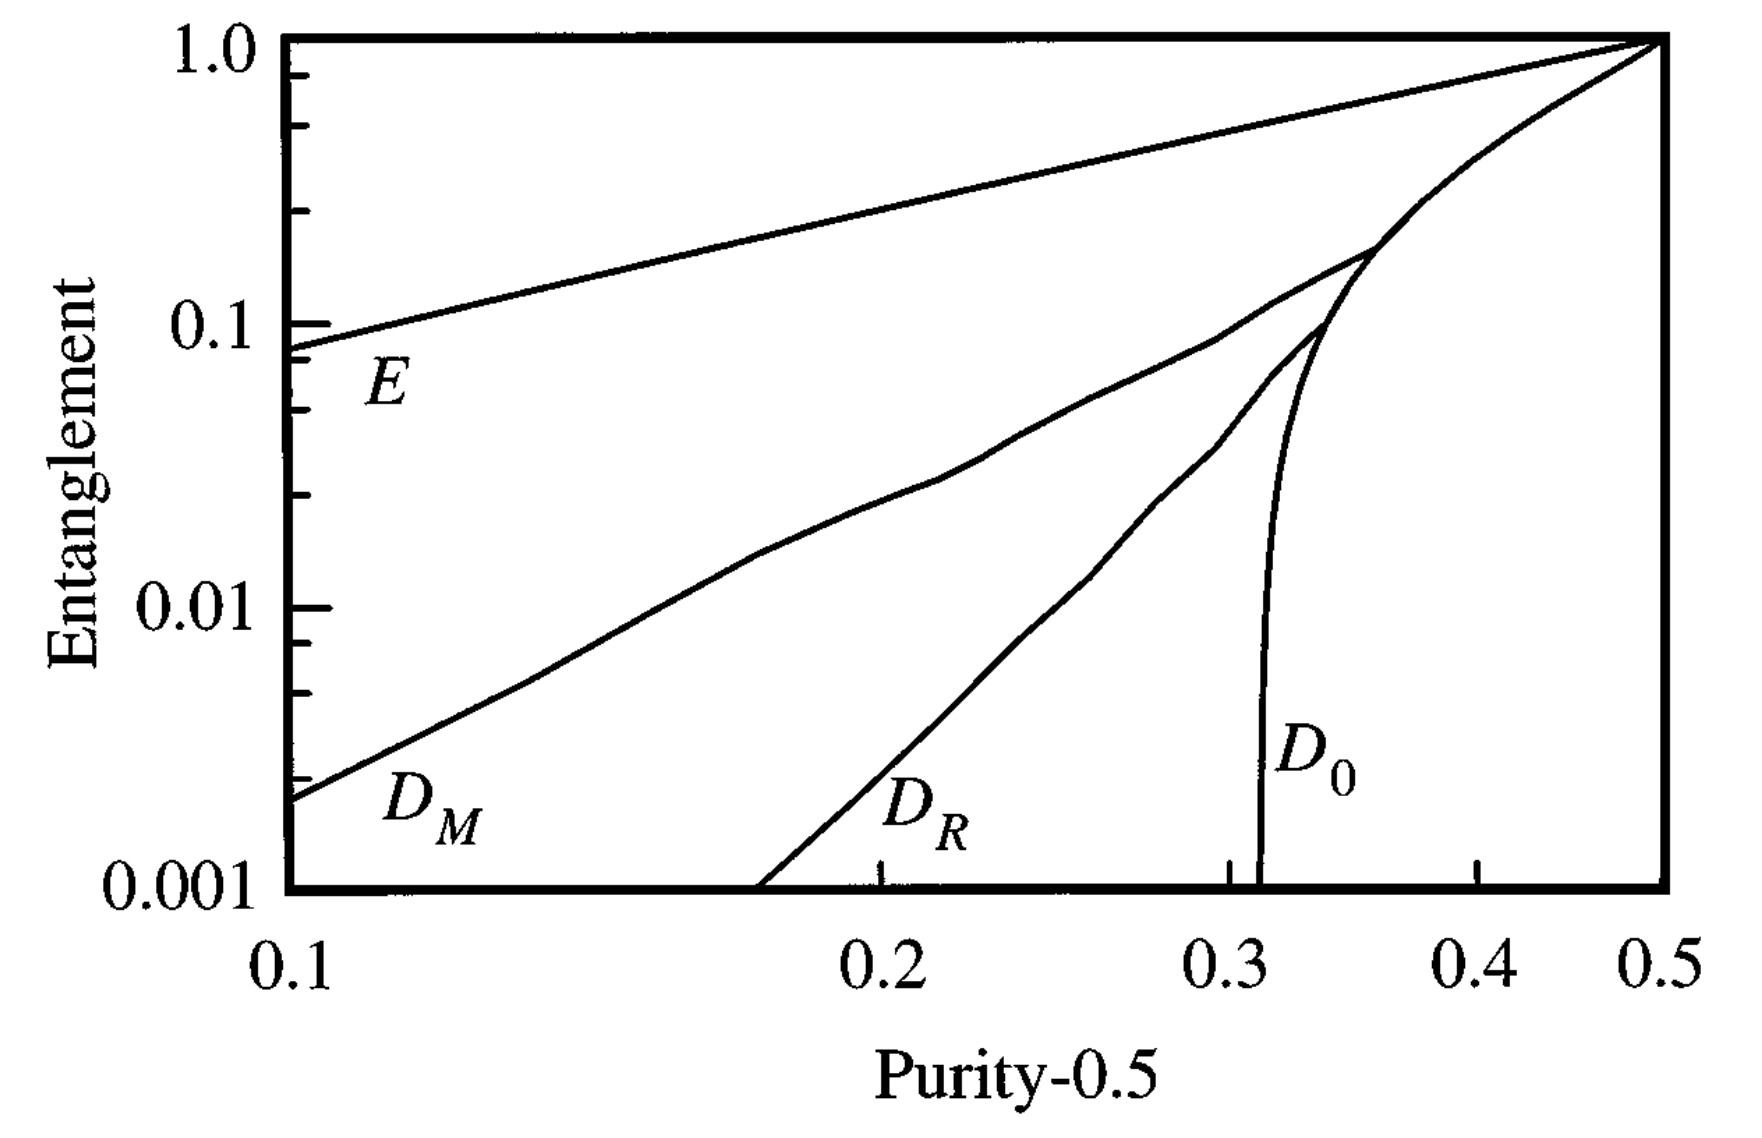
\includegraphics[width=0.7\textwidth]{image/figure_1.png}
    \caption{Log-log plot of entanglement distillable form $W_F$ ($D_0$: breeding method만 사용, $D_R$: breeding method + recurrence method, $D_M$: breeding method + 베이스라인, $E$: upper bound)}
    \label{fig:plot}
\end{figure}

본 논문에서 제안하는 방법은 QEC 없이도 noisy channel을 사용하여 $\Phi^+$를 얻는 방법과 얻어낸 pure $\Phi^+$를 사용하여 더 많은 $\Phi^+$를 만들어내는 프로토콜이다. 또한 mixed state의 entanglement를 표현하기 위한 2가지 measure Distillable entanglement $D(M)$, 그리고 entanglement of formation $E(W_F)$을 소개한다.
\section{Practical usefulness of the article}
\begin{kaobox}
    \textit{Argue the practical usefulness of the results.}
\end{kaobox}
이 논문에서는 quantum error correction(QEC)을 사용하는 대신, quantum channel을 이용하여 pure Bell state를 생성하고 이를 복제하는 방법을 소개한다. 현재 QEC는 arbitrary single qubit error를 정정할 수 있는 logical qubit \textbf{1개}를 나타내기 위해서 \textbf{최소 5개}의 physical qubit이 필요하며, 따라서 qubit의 개수에 크게 의존적이다.
그러나 본 논문에서 제안하는 방법을 도입하면 충분한 반복을 통해 qubit 개수에 제한 없이 purification을 수행할 수 있다.\sidenote[][]{breeding method 제외}

\pagebreak
이러한 기여를 바탕으로 본 논문에서 제안하는 protocol을 이용하면 다음과 같은 분야에서 활용할 수 있으리라고 기대한다.
\begin{itemize}
    \item \textbf{Quantum teleportation}: Quantum teleportation을 위해서 필요한 Bell state의 공유 과정에서 noisy channel 때문에 발생하는 noise를 제거할 수 있으므로 보다 정확한 quantum teleportation을 수행할 수 있다. 
    \item \textbf{QKD}: Quantum Key Distribution에서 entanglement를 기반으로 하는 protocol에서는 secret key를 공유할 사람들이 Bell state를 공유해야한다. 따라서 본 논문에서 제안하는 protocol을 도입하여 QKD에서의 오류 완화에 사용될 수 있다.
    \item \textbf{Fault-tolerant quantum communication}: QEC와 같은 기존의 noise 완화 방법과 결합하여 더 높은 수준의 오류 완화 및 정정 방법을 고안할 수 있다.
    \item \textbf{Measure}: mixed state의 entanglement를 나타내기 위해 사용될 수 있는 두 가지 지표, $E(W_F), D(M)$을 제안함으로서 추후 quantum information theory의 연구에서 사용할 수 있도록 기여한다.
\end{itemize}

% \appendix % From here onwards, chapters are numbered with letters, as is the appendix convention
% \section{Appendix}
% \blindtext

%----------------------------------------------------------------------------------------
%	BIBLIOGRAPHY
%----------------------------------------------------------------------------------------

% The bibliography needs to be compiled with biber using your LaTeX editor, or on the command line with 'biber main' from the template directory

\printbibliography[title=Bibliography] % Set the title of the bibliography and print the references

\end{document}